\chapter{Kloosterman Sums: Vertical Sato Tate and Random Fourier Series}\label{ch:06b}

In 1926 Kloosterman, counting representations of integers by quaternary quadratic forms with the circle method, met the exponential sums that now bear his name and proved that they are smaller than trivial by a power of the modulus \cite{kloosterman1926}. Twenty two years later Weil deduced the optimal bound from the Riemann hypothesis for curves over finite fields \cite{weil1948b}, and forty years after that Katz determined the statistical law of the normalised sums: as the prime grows, Kloosterman angles are distributed like the angles of Haar random matrices in $\SU(2)$ \cite{katz1988}. The same semicircle that governs Frobenius traces of elliptic curves (Chapter~\ref{ch:04}) and the eigenvalues of random matrices (Chapter~\ref{ch:06}) thus governs a family of exponential sums with no elliptic curve in sight. Kloosterman sums are also tied to the spectral theory of automorphic forms: the Bruggeman Kuznetsov formula equates sums of them with spectral averages of Fourier coefficients of Maass forms, and Selberg's bound $\lambda_1\ge 3/16$ is Weil's bound read spectrally. In the last part of the chapter we follow Kowalski and Sawin \cite{kowalskisawin2016}, who joined partial Kloosterman sums into polygonal paths and found in the limit a random Fourier series with independent Sato Tate coefficients. We prove the analytic reduction behind their theorem, compute the covariance of the limit in closed form, and show exactly how a change of parametrisation removes one Sato Tate coefficient from the limit, the effect behind a variance deficit of $1/\pi^2$ that our computations ran into.

\section{Kloosterman sums and Weil's bound}\label{sec:06bweil}

Let $p$ be an odd prime and write $e(z)=e^{2\pi iz}$. For $x\in\mathbb{F}_p^\times$ let $\bar x$ denote its inverse. For $a,b\in\mathbb{F}_p$ the \emph{Kloosterman sum}\index{Kloosterman sum} is
\[
\mathrm{Kl}(a,b;p)=\sum_{x\in\mathbb{F}_p^\times}e\Bigl(\frac{ax+b\bar x}{p}\Bigr),
\]
and we abbreviate $\mathrm{Kl}(c;p)=\mathrm{Kl}(c,1;p)$. Three elementary properties are used constantly (Exercise~\ref{ex:06bbasic}). First, $\mathrm{Kl}(a,b;p)$ is real, because $x\mapsto -x$ maps the sum to its complex conjugate. Second, if $a\ne0$ the substitution $y=ax$ gives $\mathrm{Kl}(a,b;p)=\mathrm{Kl}(1,ab;p)$, so the sum depends only on the product $ab$ when $a\neq 0$; by symmetry the same holds when $b\ne0$, so $\mathrm{Kl}(a,b;p)=\mathrm{Kl}(ab;p)$ unless $a=b=0$. Third, if exactly one of $a,b$ vanishes the sum is a Ramanujan sum: $\sum_{x\neq0}e(cx/p)=-1$ for $c\ne0$, so $\mathrm{Kl}(0;p)=-1$.

The trivial bound is $|\mathrm{Kl}(a;p)|\le p-1$. The moments show that the typical size is $\sqrt p$.

\begin{proposition}[Second and fourth moments]\label{prop:06bmoments}
For every odd prime $p$,
\begin{gather*}
\sum_{a\in\mathbb{F}_p^\times}\mathrm{Kl}(a;p)=1,\qquad
\sum_{a\in\mathbb{F}_p^\times}\mathrm{Kl}(a;p)^2=p^2-p-1,\\
\sum_{a\in\mathbb{F}_p^\times}\mathrm{Kl}(a;p)^4=2p^3-3p^2-3p-1 .
\end{gather*}
Consequently the normalised values $x_{p,a}=\mathrm{Kl}(a;p)/\sqrt p$ have empirical second moment $1-1/(p(p-1))$ and empirical fourth moment $2-1/p+O(p^{-2})$ over $a\in\mathbb{F}_p^\times$.
\end{proposition}

These identities are classical; we include the proof because the fourth moment is the first place where the semicircle appears.

\begin{proof}
We sum over all $a\in\mathbb{F}_p$ and subtract the term $a=0$, where $\mathrm{Kl}(0;p)=-1$. By orthogonality of additive characters, $\sum_ae(au/p)=p\,\mathbb{I}_{u=0}$, we have $\sum_a\mathrm{Kl}(a;p)=\sum_{x\ne0}e(\bar x/p)\sum_ae(ax/p)=0$, and, since $\mathrm{Kl}(a;p)$ is real,
\[
\sum_a\mathrm{Kl}(a;p)^2=\sum_{x,y\ne0}e\Bigl(\frac{\bar x-\bar y}{p}\Bigr)\sum_ae\Bigl(\frac{a(x-y)}{p}\Bigr)=p(p-1).
\]
For the fourth moment write $\mathrm{Kl}(a;p)^2=\sum_{u}e(au/p)T(u)$ with
\[
T(u)=\sum_{\substack{x,y\ne0\\ x+y=u}}e\Bigl(\frac{\bar x+\bar y}{p}\Bigr).
\]
Since $\mathrm{Kl}^2$ is real, Parseval gives $\sum_a\mathrm{Kl}(a;p)^4=\sum_a|\mathrm{Kl}(a;p)^2|^2=p\sum_u|T(u)|^2$. For $u=0$ we have $y=-x$, hence $\bar y=-\bar x$, and $T(0)=p-1$. For $u\ne0$ we have $\bar x+\bar y=u\,\overline{x(u-x)}$, and the substitution $x=us$ gives $T(u)=\sum_{s\ne0,1}e(\bar u\,\overline{s(1-s)}/p)$. The equation $s(1-s)=v$ has $1+\bigl(\frac{1-4v}{p}\bigr)$ solutions, with $\bigl(\frac{\cdot}{p}\bigr)$ the Legendre symbol $\chi$. Writing $w=\bar v$ and using $\chi(1-4\bar w)=\chi(w(w-4))$,
\[
T(u)=-1+G(\bar u),\qquad G(c)=\sum_{w\in\mathbb{F}_p}\chi\bigl(w(w-4)\bigr)e(cw/p).
\]
Now $G(0)=\sum_w\chi(w^2-4w)=-1$ (a quadratic with nonzero discriminant), $\sum_cG(c)=p\,\chi(0)=0$, and by Parseval $\sum_c|G(c)|^2=p\,\#\{w:w(w-4)\ne0\}=p(p-2)$. Hence $\sum_{c\ne0}|G(c)|^2=p^2-2p-1$ and $\sum_{c\ne0}G(c)=1$, so
\[
\sum_{u\ne0}|T(u)|^2=\sum_{c\ne0}|G(c)-1|^2=(p^2-2p-1)-2+(p-1)=p^2-p-4 .
\]
With $T(0)^2=(p-1)^2$ added, $\sum_u|T(u)|^2=2p^2-3p-3$, so $\sum_{a\in\mathbb{F}_p}\mathrm{Kl}(a;p)^4=2p^3-3p^2-3p$, and removing $a=0$ proves the claim.
\end{proof}

The limits $1$ and $2$ are the first two even moments of the Sato Tate law $\ST$, the Catalan numbers $C_1,C_2$ of Chapter~\ref{ch:04}. The second moment shows that $\max_a|\mathrm{Kl}(a;p)|\ge\sqrt{p}\,(1+o(1))$. The fourth moment gives $\max_a|\mathrm{Kl}(a;p)|^4\le2p^3$, that is $|\mathrm{Kl}(a;p)|\le2^{1/4}p^{3/4}$, which is essentially Kloosterman's bound. A bound of the right order $p^{k+1}$ for the moment of order $2k$ would give the exponent $\frac12+\frac1{2k}$, but proving it already requires the geometry behind the optimal bound.

\begin{theorem}[Weil \cite{weil1948b}]\label{thm:06bweil}\index{Weil bound}
For $p\nmid ab$, $|\mathrm{Kl}(a,b;p)|\le 2\sqrt p$.
\end{theorem}

\paragraph{Idea of proof.} By the second property above we may take $b=1$ and $a\ne0$. For $n\ge1$ let $\mathrm{Kl}_n(a)=\sum_{x\in\mathbb{F}_{p^n}^\times}\psi\bigl(\mathrm{Tr}_{\mathbb{F}_{p^n}/\mathbb{F}_p}(ax+\bar x)\bigr)$ with $\psi(z)=e(z/p)$, so that $\mathrm{Kl}_1(a)=\mathrm{Kl}(a;p)$. To a monic $f\in\mathbb{F}_p[X]$ with $f(0)\ne0$ attach $\lambda(f)=\psi\bigl(a\sigma(f)+\sigma'(f)\bigr)$, where $\sigma(f)$ and $\sigma'(f)$ are the sums of the roots of $f$ and of their inverses. Then $\lambda$ is completely multiplicative, and grouping the $x\in\mathbb{F}_{p^n}^\times$ by their minimal polynomials over $\mathbb{F}_p$ turns the Euler product over irreducible $f$ into
\[
L_a(T)=\exp\Bigl(\sum_{n\ge1}\mathrm{Kl}_n(a)\frac{T^n}{n}\Bigr)=\sum_{f}\lambda(f)\,T^{\deg f}.
\]
For $f=X^d+c_{d-1}X^{d-1}+\dots+c_0$ we have $\sigma(f)=-c_{d-1}$ and $\sigma'(f)=-c_1/c_0$. When $d\ge3$ the coefficient $c_{d-1}$ is free and the terms of degree $d$ cancel because $a\ne0$; counting the terms of degrees $1$ and $2$ gives $L_a(T)=1+\mathrm{Kl}(a;p)\,T+pT^2$. This is Weil's argument \cite{weil1948b}. Factor $L_a(T)=(1-\alpha T)(1-\beta T)$; then $\mathrm{Kl}_n(a)=-(\alpha^n+\beta^n)$ and $\alpha\beta=p$. Counting the points of the Artin Schreier curve $y^p-y=ax+1/x$, which has genus $p-1$, over $\mathbb{F}_{p^n}$ shows that $\alpha$ and $\beta$ are among the reciprocal roots of the numerator of its zeta function, so the Riemann hypothesis for curves gives $|\alpha|=|\beta|=\sqrt p$, hence the bound. Conversely, a bound $|\mathrm{Kl}_n(a)|\le Cp^{n/2}$ with $C$ independent of $n$ already forces $|\alpha|=|\beta|=\sqrt p$ (Exercise~\ref{ex:06bweilL}). The elementary method of Stepanov \cite{stepanov1969}, in Bombieri's form \cite{bombieri1974}, proves point count bounds of exactly this kind over every extension $\mathbb{F}_{p^n}$, and so reaches the same conclusion.

Since $\alpha\beta=p$, $|\alpha|=|\beta|=\sqrt p$ and $\alpha+\beta=-\mathrm{Kl}(a;p)$ is real, we have $\beta=\bar\alpha$, and we may write $\{\alpha,\beta\}=\{-\sqrt p\,e^{i\theta},-\sqrt p\,e^{-i\theta}\}$ with a unique \emph{Kloosterman angle} $\theta_{p,a}\in[0,\pi]$, so that
\[
x_{p,a}=\frac{\mathrm{Kl}(a;p)}{\sqrt p}=2\cos\theta_{p,a}\in[-2,2].
\]
In the language of $\ell$ adic sheaves, Deligne and Katz construct a rank two lisse sheaf $\mathcal{K}l$ on $\mathbb{G}_m$ over $\mathbb{F}_p$, pure of weight one, whose Frobenius at $a\in\mathbb{F}_p^\times$ has eigenvalues $\alpha,\beta$ and trace $-\mathrm{Kl}(a;p)$ \cite{katz1988}. After the half Tate twist the Frobenius at $a$ determines a conjugacy class in $\SU(2)$, exactly like the Satake parameter $\mathrm{diag}(e^{i\theta_p},e^{-i\theta_p})$ of a modular form at a prime $p$. Kloosterman angles and Satake angles live on the same circle; the sign in the trace is immaterial for us because $\ST$ is invariant under $\theta\mapsto\pi-\theta$.

\section{Katz's theorem: vertical Sato Tate}\label{sec:06bkatz}

There are two ways to let the Kloosterman angles vary. \emph{Vertically}, fix $p$ and let $a$ run over $\mathbb{F}_p^\times$, then let $p\to\infty$. \emph{Horizontally}, fix $a$ and let $p$ run over the primes. The vertical problem is the analogue of the vertical Sato Tate theorem for Hecke eigenvalues in Chapter~\ref{ch:07}; the horizontal problem is the analogue of Sato Tate for a fixed elliptic curve.

\begin{theorem}[Katz \cite{katz1988}]\label{thm:06bkatz}\index{Katz equidistribution theorem}\index{vertical Sato Tate theorem}
As $p\to\infty$ the multisets $\{\theta_{p,a}:a\in\mathbb{F}_p^\times\}$ become equidistributed in $[0,\pi]$ with respect to the Sato Tate measure $\frac2\pi\sin^2\theta\,d\theta$. Equivalently, for every continuous $f$ on $[-2,2]$,
\[
\frac{1}{p-1}\sum_{a\in\mathbb{F}_p^\times}f\Bigl(\frac{\mathrm{Kl}(a;p)}{\sqrt p}\Bigr)\longrightarrow\int_{-2}^2f\,d\ST .
\]
\end{theorem}

Since $\mathrm{Kl}(a,b;p)=\mathrm{Kl}(ab;p)$ and $a\mapsto ab$ permutes $\mathbb{F}_p^\times$ when $p\nmid b$, the same holds for $\mathrm{Kl}(a,b;p)$ with $b$ fixed.

\paragraph{Proof sketch.} By the Weyl criterion (Theorem~\ref{thm:04weyl}, whose proof applies verbatim to any sequence of probability measures on $[0,\pi]$) it suffices to show that the averages of $U_n(\cos\theta_{p,a})$ tend to zero for each $n\ge1$. Up to the sign $(-1)^n$, $U_n(\cos\theta_{p,a})$ is the trace of Frobenius at $a$ on $\Sym^n$ of the normalised sheaf. By the Grothendieck Lefschetz trace formula,
\[
\sum_{a\in\mathbb{F}_p^\times}\tr\bigl(\Frob_a\mid\Sym^n\mathcal{K}l\bigr)=\sum_{i=0}^2(-1)^i\tr\bigl(\Frob\mid H^i_c(\mathbb{G}_{m,\bar{\mathbb{F}}_p},\Sym^n\mathcal{K}l)\bigr).
\]
The group $H^0_c$ vanishes because $\mathbb{G}_m$ is affine. The group $H^2_c$ is the space of coinvariants of the geometric monodromy group acting on $\Sym^n$, and Katz proved that this group is $\SL_2$ \cite{katz1988}. The inputs are local: the sheaf has geometrically trivial determinant, it is tamely ramified at $0$ with unipotent local monodromy consisting of a single Jordan block, and it is wildly ramified at $\infty$ with both breaks equal to $\frac12$ (Swan conductor $1$); Katz deduces from them that no proper subgroup of $\SL_2$ can be the geometric monodromy group. Since $\Sym^n$ is an irreducible nontrivial representation of $\SL_2$ for $n\ge1$, the coinvariants vanish. Finally, by Deligne's Weil II \cite{deligne1980} the eigenvalues of Frobenius on $H^1_c$ have absolute value at most $\sqrt p$ after normalisation, and the Grothendieck Ogg Shafarevich formula gives $\dim H^1_c=\mathrm{Swan}_\infty(\Sym^n\mathcal{K}l)\le\frac{n+1}2$, because $\Sym^n\mathcal{K}l$ is tame at $0$ and its breaks at $\infty$ are at most $\frac12$. Therefore
\[
\Bigl|\frac{1}{p-1}\sum_{a\in\mathbb{F}_p^\times}U_n(\cos\theta_{p,a})\Bigr|\le\frac{(n+1)\sqrt p}{2(p-1)}\le\frac{n+1}{\sqrt p}.
\]

This is Deligne's equidistribution theorem \cite{deligne1980} applied to the Kloosterman sheaf, and the monodromy computation is the heart of the matter; Katz and Sarnak use exactly this mechanism to produce the random matrix statistics of Chapter~\ref{ch:06} \cite{katzsarnak1999}. The bound $(n+1)/\sqrt p$ for the Weyl sums gives an explicit rate in the discrepancy, worked out by Niederreiter \cite{niederreiter1991}. Katz also computed the monodromy of the hyper Kloosterman sheaves of rank $n$: it is the symplectic group $\mathrm{Sp}_n$ for even $n$, and $\SL_n$ for odd $n$ when $p$ is odd \cite{katz1988}. The case $n=2$ of this chapter is the first member of the symplectic series, since $\SL_2=\mathrm{Sp}_2$ and $\SU(2)=\USp(2)$.

For the paths of Section~\ref{sec:06bpaths} we need a joint statement for additive shifts.

\begin{theorem}[Joint equidistribution of shifts]\label{thm:06bjoint}
Let $h_1,\dots,h_k$ be distinct integers. As $p\to\infty$, with $a$ uniform among the elements of $\mathbb{F}_p$ for which $a+h_j\ne0$ for all $j$, the random vector $\bigl(\mathrm{Kl}(a+h_1;p),\dots,\mathrm{Kl}(a+h_k;p)\bigr)/\sqrt p$ converges in law to $(\mathrm{ST}_1,\dots,\mathrm{ST}_k)$, independent random variables with law $\ST$.
\end{theorem}

This is due to Kowalski and Sawin \cite{kowalskisawin2016}, who deduce it from Katz's computation of the monodromy. The relevant monodromy group is now that of the direct sum of the translated sheaves $[x\mapsto x+h_j]^*\mathcal{K}l$, a subgroup of $\SL_2^k$ projecting onto each factor. By the Goursat Kolchin Ribet criterion \cite{katz1990}\index{Goursat Kolchin Ribet criterion} it is all of $\SL_2^k$ unless two of the translates become geometrically isomorphic after tensoring with a rank one sheaf. The ramification at $0$ rules this out. Pulling back by $x\mapsto x-h_i$, we may compare $\mathcal{K}l$ itself with its translate $[x\mapsto x+h]^*\mathcal{K}l$, where $h=h_j-h_i\neq0$, and an isomorphism $[x\mapsto x+h]^*\mathcal{K}l\simeq\mathcal{K}l\otimes\mathcal{L}$ is impossible: the translate is lisse at $0$, while $\mathcal{K}l\otimes\mathcal{L}$ is ramified at $0$ for every rank one sheaf $\mathcal{L}$, because the local monodromy of $\mathcal{K}l$ at $0$ is a nontrivial unipotent block. Joint equidistribution then follows from Deligne's theorem with $\SU(2)^k$ in place of $\SU(2)$: the Kloosterman sums at distinct additive shifts behave like independent traces of Haar random matrices.

\subsection{Data}

For this book we computed $\mathrm{Kl}(a;p)=\sum_{x=1}^{p-1}e((x+a\bar x)/p)$ for all $a$ at $p=1009$ and $p=10007$, and for $3000$ random $a$ at $p=100003$. Table~\ref{tab:06bkatz} compares the even moments of $\mathrm{Kl}/\sqrt p$ with the Catalan numbers. The second and fourth moments at $p=1009$ and $p=10007$ agree with the exact values of Proposition~\ref{prop:06bmoments} to all printed digits: for $p=1009$ the identity predicts $1-1/(1009\cdot1008)=0.999999$ and $(2p^3-3p^2-3p-1)/((p-1)p^2)=1.999005$. The largest values of $|\mathrm{Kl}|/\sqrt p$ are $1.98077$ and $1.99876$, inside Weil's interval and close to its edge, and Kolmogorov Smirnov tests against $\ST$ give $p$ values $0.918$ and $0.993$ (descriptive only, since the values $\mathrm{Kl}(a;p)$ are not independent samples). Figure~\ref{fig:06bkatz} shows the histogram at $p=10007$.

\begin{table}[t]\centering\small
\begin{tabular}{lcccc}
\toprule
& $m=1$ & $m=2$ & $m=3$ & $m=4$\\
\midrule
$p=1009$, all $a$ & $0.999999$ & $1.99900$ & $4.98271$ & $13.90784$\\
$p=10007$, all $a$ & $1.0000000$ & $1.99990$ & $5.00198$ & $14.03501$\\
$p=100003$, $3000$ values & $0.9918$ & $1.9794$ & $4.9547$ & $13.9179$\\
Catalan $C_m$ & $1$ & $2$ & $5$ & $14$\\
\bottomrule
\end{tabular}
\caption{Empirical moments $\E(\mathrm{Kl}(a;p)/\sqrt p)^{2m}$, with $a$ uniform over the values listed, against the Sato Tate moments $C_m$. For the random sample at $p=100003$ the standard errors under $\ST$, $\bigl((C_{2m}-C_m^2)/3000\bigr)^{1/2}$, are about $0.02$, $0.06$, $0.19$ and $0.64$ in the four columns.}\label{tab:06bkatz}
\end{table}

\begin{figure}[t]\centering
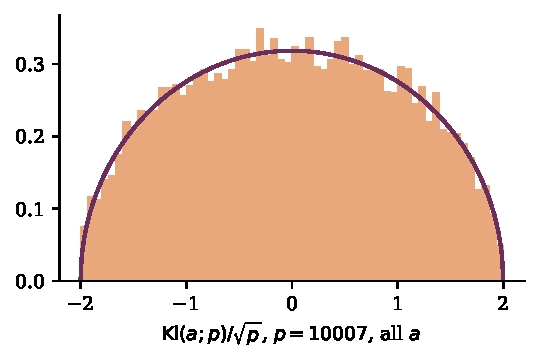
\includegraphics[width=0.62\textwidth]{figs/kloosterman_katz.pdf}
\caption{Histogram of the normalised Kloosterman sums $\mathrm{Kl}(a;p)/\sqrt p$ for all $a\in\mathbb{F}_p^\times$, $p=10007$, against the semicircle density $\frac1{2\pi}\sqrt{4-x^2}$ of $\ST$ (Theorem~\ref{thm:06bkatz}).}\label{fig:06bkatz}
\end{figure}

\subsection{The horizontal question}

For a fixed holomorphic newform of weight at least $2$ with trivial character and without complex multiplication, Sato Tate in the horizontal direction is a theorem (Theorem~\ref{thm:04STthm}), because the Satake parameters at varying $p$ are the local components of a single global automorphic representation, and the potential automorphy \cite{blght2011} and then automorphy \cite{newtonthorne2021,newtonthorne2021b} of its symmetric powers supply $L$ functions holomorphic and nonvanishing on $\Re s\ge1$ (Chapter~\ref{ch:04}). For Kloosterman sums there is no such global object: as $p$ varies, the sheaves $\mathcal{K}l$ live over different finite fields and are not known to be the reductions of a compatible system attached to a motive or automorphic representation over $\Q$. Katz conjectured the horizontal law nevertheless.

\begin{conjecture}[Katz's horizontal conjecture]\label{conj:06bhorizontal}\index{Katz horizontal conjecture}
Fix a nonzero integer $a$. As $p$ runs over the odd primes not dividing $a$, ordered by size, the angles $\theta_{p,a}$ are equidistributed in $[0,\pi]$ with respect to $\frac2\pi\sin^2\theta\,d\theta$. Equivalently,
\[
\frac{1}{\pi(x)}\sum_{p\le x,\ p\nmid a}U_n\Bigl(\frac{\mathrm{Kl}(a;p)}{2\sqrt p}\Bigr)\longrightarrow0\qquad(n\ge1).
\]
\end{conjecture}

Very little is known. Even the statement that $\mathrm{Kl}(1;p)$ is positive for infinitely many primes and negative for infinitely many primes is, to our knowledge, open; Fouvry and Michel proved sign changes of $\mathrm{Kl}(1;c)$ along moduli $c$ with a bounded number of prime factors \cite{fouvrymichel2007}, using sieve methods together with Katz's equidistribution results. The vertical theorem, by contrast with the horizontal conjecture, is geometry over a single finite field.

\section{Kloosterman sums and automorphic forms}\label{sec:06bkuznetsov}

For an integer $c\ge1$ let $S(m,n;c)=\sum_{x\in(\Z/c\Z)^\times}e((mx+n\bar x)/c)$. For prime $c=p$ this is $\mathrm{Kl}(m,n;p)$. The Chinese remainder theorem gives a twisted multiplicativity, and Weil's bound together with an elementary evaluation at prime powers yields
\[
|S(m,n;c)|\le\tau(c)\,(m,n,c)^{1/2}\,c^{1/2},
\]
with $\tau$ the divisor function \cite{iwanieckowalski2004}.

\subsection{The Bruggeman Kuznetsov formula}

Let $\{u_j\}$ be an orthonormal basis of Maass cusp forms for $\SL_2(\Z)$, eigenfunctions of the hyperbolic Laplacian with eigenvalues $\lambda_j=\frac14+t_j^2$, with Fourier expansions $u_j(z)=\sum_{n\ne0}\rho_j(n)W_{s_j}(nz)$, where $s_j=\frac12+it_j$ and $W_s(z)=2y^{1/2}K_{s-1/2}(2\pi y)e(x)$ is the Whittaker function, as in \cite{iwaniec2002}. Put $\nu_j(n)=(4\pi|n|/\cosh\pi t_j)^{1/2}\rho_j(n)$.

\begin{theorem}[Bruggeman \cite{bruggeman1978}, Kuznetsov \cite{kuznetsov1980}]\label{thm:06bkuznetsov}\index{Bruggeman Kuznetsov formula}
Let $\delta>0$ and let $h$ be even and holomorphic in $|\Im t|\le\frac12+\delta$ with $h(t)\ll(1+|t|)^{-2-\delta}$. For integers $m,n\ge1$,
\begin{multline*}
\sum_j h(t_j)\overline{\nu_j(m)}\nu_j(n)+\frac{1}{4\pi}\int_{-\infty}^{\infty}h(t)\,\overline{\eta_m(t)}\eta_n(t)\,dt\\
=\frac{\delta_{m,n}}{\pi}\int_{-\infty}^\infty t\tanh(\pi t)h(t)\,dt+\sum_{c\ge1}\frac{S(m,n;c)}{c}\,h^+\Bigl(\frac{4\pi\sqrt{mn}}{c}\Bigr),
\end{multline*}
where $\eta_n(t)=(4\pi|n|/\cosh\pi t)^{1/2}\rho_t(n)$, with $\rho_t(n)$ the coefficient of $W_{1/2+it}(nz)$ in the Eisenstein series $E(z,\frac12+it)$, and
\[
h^+(x)=2i\int_{-\infty}^\infty J_{2it}(x)\frac{h(t)\,t}{\cosh\pi t}\,dt .
\]
\end{theorem}

The normalisation of $W_s$, $\rho_j$, $\nu_j$ and of $E(z,s)=\sum_{\gamma\in\Gamma_\infty\backslash\SL_2(\Z)}\operatorname{Im}(\gamma z)^s$ is that of Iwaniec \cite{iwaniec2002}. Constants differ between sources: dividing by $\pi$ gives the equivalent form with spectral weights $\overline{a_j(m)}a_j(n)/\cosh\pi t_j$, where $a_j(n)=2|n|^{1/2}\rho_j(n)$ is the coefficient of $y^{1/2}K_{it_j}(2\pi|n|y)e(nx)$, diagonal constant $\pi^{-2}$ and prefactor $2i/\pi$ in $h^+$. The formula holds for congruence subgroups $\Gamma_0(N)$ with $c$ restricted to multiples of $N$. Its structure parallels the trace formula picture of Chapter~\ref{ch:07}. The left side is a spectral average of products of Fourier coefficients, that is of Hecke eigenvalues, since $\nu_j(n)=\nu_j(1)\lambda_j(n)$ for a basis of Hecke eigenforms, with $\lambda_j(n)$ the eigenvalues normalised so that the Ramanujan conjecture reads $|\lambda_j(p)|\le2$. The diagonal term $\delta_{m,n}$ carries the archimedean Plancherel density $t\tanh(\pi t)$, the analogue of the Kesten McKay density $\mu_q$, and the Kloosterman terms are the analogue of the cycle counts that measure the deviation of a finite quotient from its universal cover. The formula can be read in either direction: as a tool for averaging Fourier coefficients (the Kloosterman side is small by Weil), or as a tool for bounding sums of Kloosterman sums (the spectral side is controlled). The second reading is Kuznetsov's.

\subsection{Selberg's 3/16 theorem}

Let $\Gamma=\Gamma_0(N)$ and let $\lambda_1(\Gamma)$ be the smallest nonzero eigenvalue of the Laplacian on $L^2(\Gamma\backslash\mathbb{H})$. The continuous spectrum begins at $\frac14$, the bottom of the spectrum of the hyperbolic plane itself; an eigenvalue $\lambda=s(1-s)<\frac14$ with $\frac12<s<1$ is called exceptional.

\begin{theorem}[Selberg \cite{selberg1965}]\label{thm:06bselberg}\index{Selberg 3/16 theorem}
For every congruence subgroup $\Gamma_0(N)$, $\lambda_1\ge\frac{3}{16}$.
\end{theorem}

\paragraph{Sketch of Selberg's argument.} Consider the Kloosterman zeta function
\[
Z_{m,n}(s)=\sum_{c\equiv0\ (N)}\frac{S(m,n;c)}{c^{2s}} .
\]
Selberg showed, by unfolding the inner product of two Poincar\'e series and inserting the spectral decomposition, that $Z_{m,n}$ continues meromorphically, and that in $\Re s>\frac12$ its only possible poles are at the points $s_j\in(\frac12,1)$ with $s_j(1-s_j)$ an exceptional eigenvalue, with residue a nonzero multiple of $\sum\overline{\rho(m)}\rho(n)$ summed over an orthonormal basis of that eigenspace. Taking $m=n$ with $\rho(n)\ne0$ for some form in the eigenspace, the residue is a positive multiple of $\sum|\rho(n)|^2$, so the pole is genuine. On the other hand Weil's bound gives $|S(n,n;c)|\ll_{n,\varepsilon} c^{1/2+\varepsilon}$, so the series converges absolutely for $\Re s>\frac34$ and $Z_{n,n}$ is holomorphic there. Hence every exceptional $s_j$ satisfies $s_j\le\frac34$, and since $s\mapsto s(1-s)$ decreases on $[\frac12,1]$, $\lambda_j\ge\frac34\cdot\frac14=\frac3{16}$.

Selberg conjectured that $\lambda_1\ge\frac14$ for all congruence subgroups. In representation theoretic language this is the Ramanujan conjecture at the archimedean place for Maass forms: the archimedean component of the automorphic representation is tempered exactly when $\lambda\ge\frac14$. The best bound known is due to Kim and Sarnak in the appendix to Kim's paper \cite{kimsarnak2003}: using the automorphy of $\Sym^4$ for $\GL_2$, they show that the archimedean Satake parameter of a Maass cusp form on a congruence subgroup has real part at most $\frac7{64}$, hence $\lambda_1\ge\frac14-\bigl(\frac{7}{64}\bigr)^2=\frac{975}{4096}\approx0.238$. Earlier improvements on $\frac3{16}$ were obtained by Luo, Rudnick and Sarnak \cite{lrs1995} and by Kim and Shahidi \cite{kimshahidi2002}.

\subsection{Linnik and Selberg on sums of Kloosterman sums}

Weil's bound alone gives $\sum_{c\le x}|S(m,n;c)|/c\ll x^{1/2+\varepsilon}$. Linnik \cite{linnik1962} and Selberg \cite{selberg1965} conjectured that the signs of the Kloosterman sums cancel as $c$ varies.

\begin{conjecture}[Linnik, Selberg]\label{conj:06blinnik}\index{Linnik Selberg conjecture}
For fixed $m,n\ge1$ and every $\varepsilon>0$,
\[
\sum_{c\le x}\frac{S(m,n;c)}{c}\ll_{m,n,\varepsilon}x^{\varepsilon}.
\]
\end{conjecture}

Kuznetsov proved the bound $x^{1/6+\varepsilon}$ \cite{kuznetsov1980}, and to our knowledge the exponent $\frac16$ has not been improved for fixed $m,n$. He obtained it from the version of Theorem~\ref{thm:06bkuznetsov} read in the opposite direction, in which a test function on the Kloosterman side is prescribed (here one that approximates the indicator of $c\le x$) and the spectral side is bounded \cite{iwanieckowalski2004}. The connection with Theorem~\ref{thm:06bselberg} is direct. If the analogue of Conjecture~\ref{conj:06blinnik} held for $\Gamma_0(N)$, with $c$ restricted to multiples of $N$, then partial summation would make $Z_{n,n}(s)$ holomorphic in $\Re s>\frac12$, and Selberg's argument would exclude exceptional eigenvalues altogether. Conversely, an exceptional eigenvalue $s_j(1-s_j)$ produces a term of order $x^{2s_j-1}$ in the smoothed sums.

\paragraph{The probabilistic reading.} Think of $c\mapsto S(m,n;c)/\sqrt c$ as a sequence of random variables. For prime $c$ these are $2\cos\theta_{c,mn}$, and if the angles behaved like independent Sato Tate variables (the horizontal model of Conjecture~\ref{conj:06bhorizontal}) the sum $\sum_{p\le x}2\cos\theta_{p,mn}/\sqrt p$ would have mean zero and variance $\sum_{p\le x}1/p\sim\log\log x$, comfortably inside $x^\varepsilon$. Square root cancellation in sums of Kloosterman sums is therefore the statement that this sequence has no drift, and Theorem~\ref{thm:06bkuznetsov} identifies the possible drifts: they are the exceptional eigenvalues, each contributing a deterministic term $x^{2s_j-1}$. The analogy with Chapters~\ref{ch:07} and~\ref{ch:08} is close. There, a connected finite quotient of the tree is Ramanujan exactly when the return probabilities of simple random walk on it approach equilibrium at an exponential rate no slower than the Kesten rate $2\sqrt q/(q+1)$ (Proposition~\ref{prop:08three}); here, $\lambda_1\ge\frac14$ means that Brownian motion on $\Gamma\backslash\mathbb{H}$, with generator the Laplacian, mixes at least at the rate $e^{-t/4}$ dictated by the spectrum of the hyperbolic plane. In both settings the Ramanujan property is a spectral gap, and a trace formula converts it into cancellation in an arithmetic sum: counts of closed nonbacktracking walks in the first case, through the Ihara Bass formula, and Kloosterman sums over moduli in the second, through Kuznetsov's.

\section{Kloosterman paths}\label{sec:06bpaths}

Kowalski and Sawin \cite{kowalskisawin2016} asked what the partial sums of a Kloosterman sum look like. For $a\in\mathbb{F}_p^\times$ and $0\le t\le1$ let
\[
S_p(a,t)=\frac{1}{\sqrt p}\sum_{1\le x\le t(p-1)}e\Bigl(\frac{ax+\bar x}{p}\Bigr),
\]
and let $K_p(a,\cdot)\in C([0,1])$ be the polygonal path that interpolates linearly between the values at $t=j/(p-1)$, $0\le j\le p-1$. Then $K_p(a,0)=0$, $K_p(a,1)=\mathrm{Kl}(a;p)/\sqrt p$, and $|K_p(a,t)-S_p(a,t)|\le p^{-1/2}$, so the two have the same limiting finite dimensional distributions. With $a$ uniform in $\mathbb{F}_p^\times$, $K_p$ is a random continuous function.\index{Kloosterman path}

\begin{definition}\label{def:06bK}
Let $(\mathrm{ST}_h)_{h\in\Z}$ be independent random variables with law $\ST$ and put $c_0(t)=t$ and $c_h(t)=(e(ht)-1)/(2\pi ih)$ for $h\ne0$. The \emph{Kloosterman random Fourier series} is
\[
K(t)=\sum_{h\in\Z}c_h(t)\,\mathrm{ST}_h=t\,\mathrm{ST}_0+\sum_{h\ne0}\frac{e(ht)-1}{2\pi ih}\mathrm{ST}_h ,
\]
the series being the limit of its symmetric partial sums over $|h|\le H$ as $H\to\infty$.
\end{definition}

Since $\E\,\mathrm{ST}_h=0$, $\E\,\mathrm{ST}_h^2=1$ and $\sum_h|c_h(t)|^2<\infty$, the series converges in $L^2$ and almost surely for each $t$. Kowalski and Sawin show, with Kahane's theory of random Fourier series, that $K$ is almost surely continuous, indeed H\"older continuous of every order below $\frac12$, and almost surely nowhere differentiable \cite{kowalskisawin2016}; so $K$ is a random element of $C([0,1])$. Since $c_h(t)=\int_0^te(hu)\,du$, the process $K$ is formally the integral $\int_0^tW(u)\,du$ of the random Fourier series $W(u)=\sum_h\mathrm{ST}_he(hu)$, whose Fourier coefficients are independent Sato Tate variables. Equivalently $c_h(t)=\overline{\widehat{\mathbb{I}_{[0,t]}}(h)}$, where $\hat f(h)=\int_0^1f(u)e(-hu)\,du$, and in this form the coefficients arise from the discrete Fourier analysis of an interval, as we now show.

\subsection{The completion formula}

\begin{lemma}[Completion]\label{lem:06bcompletion}\index{completion method}
Let $I=\{1,\dots,m\}$ with $m=\lfloor t(p-1)\rfloor$ and, for $h\in\Z$,
\[
\alpha_p(h,t)=\frac1p\sum_{y=1}^me\Bigl(\frac{hy}{p}\Bigr).
\]
Then, for every $a\in\mathbb{F}_p$,
\begin{equation}\label{eq:06bcompletion}
S_p(a,t)=\sum_{|h|<p/2}\alpha_p(h,t)\,\frac{\mathrm{Kl}(a-h;p)}{\sqrt p}.
\end{equation}
Further $\alpha_p(0,t)=m/p$, $|\alpha_p(h,t)|\le 1/(2|h|)$ for $1\le|h|<p/2$, and $\alpha_p(h,t)\to c_h(t)$ as $p\to\infty$ for each fixed $h$ and $t$.
\end{lemma}

\begin{proof}
By finite Fourier inversion on $\Z/p\Z$, for every residue $x$,
\[
\mathbb{I}_I(x)=\sum_{h\bmod p}\alpha_p(h,t)\,e\Bigl(-\frac{hx}{p}\Bigr),
\]
since $\sum_h\alpha_p(h,t)e(-hx/p)=p^{-1}\sum_{y\in I}\sum_he(h(y-x)/p)$ and the inner sum is $p$ when $y=x$ and $0$ otherwise. Insert this into the definition of $S_p$ and interchange the sums:
\begin{align*}
\sqrt p\,S_p(a,t)&=\sum_{h\bmod p}\alpha_p(h,t)\sum_{x\in\mathbb{F}_p^\times}e\Bigl(\frac{(a-h)x+\bar x}{p}\Bigr)\\
&=\sum_{h\bmod p}\alpha_p(h,t)\,\mathrm{Kl}(a-h;p);
\end{align*}
then represent the residues $h$ by $|h|<p/2$. For $h\ne0$ the geometric sum gives $|\sum_{y=1}^me(hy/p)|=|\sin(\pi hm/p)/\sin(\pi h/p)|\le1/|\sin(\pi h/p)|$, and $\sin(\pi u)\ge2u$ for $0\le u\le\frac12$ gives $|\alpha_p(h,t)|\le 1/(2|h|)$. Finally $\alpha_p(h,t)$ is a Riemann sum for $\int_0^{m/p}e(hu)\,du$ with mesh $1/p$, and $m/p\to t$, so $\alpha_p(h,t)\to\int_0^te(hu)\,du=c_h(t)$.
\end{proof}

Formula \eqref{eq:06bcompletion} is the starting point of Kowalski and Sawin \cite{kowalskisawin2016}. Its term $h\equiv a$ involves $\mathrm{Kl}(0;p)=-1$; it is the only one that is not a genuine Kloosterman sum, and for $1\le a\le p-1$ its coefficient is at most $1/(2\min(a,p-a))$ in absolute value. The completion formula exhibits the path as a linear functional of the shifted sums $\mathrm{Kl}(a-h;p)$, $|h|<p/2$, which by Theorem~\ref{thm:06bjoint} are asymptotically independent Sato Tate variables. Renaming $h\mapsto-h$ writes the same identity with the shifts $\mathrm{Kl}(a+h;p)$ and the limiting coefficients $c_{-h}(t)$; the law of $K$ is unchanged because the $\mathrm{ST}_h$ are independent and identically distributed.

The next lemma controls the tail of \eqref{eq:06bcompletion} uniformly in $p$; it uses only orthogonality.

\begin{lemma}[Uniform tail bound; this book]\label{lem:06btail}
For every $H\ge1$, every $p>2H+1$ and every $t\in[0,1]$,
\[
\frac{1}{p-1}\sum_{a\in\mathbb{F}_p^\times}\Bigl|\sum_{H<|h|<p/2}\alpha_p(h,t)\frac{\mathrm{Kl}(a-h;p)}{\sqrt p}\Bigr|^2\le\frac1H .
\]
\end{lemma}

\begin{proof}
For $k\in\mathbb{F}_p$, orthogonality in $c$ gives
\begin{align*}
\sum_{c\in\mathbb{F}_p}\mathrm{Kl}(c;p)\mathrm{Kl}(c+k;p)&=\sum_{x,y\ne0}e\Bigl(\frac{\bar x+\bar y+ky}{p}\Bigr)\sum_ce\Bigl(\frac{c(x+y)}{p}\Bigr)\\
&=p\sum_{x\ne0}e\Bigl(-\frac{kx}{p}\Bigr),
\end{align*}
which is $p(p-1)$ for $k=0$ and $-p$ for $k\ne0$. Hence, since the $\mathrm{Kl}(c;p)$ are real, for any coefficients $\beta_h$ indexed by a set $\mathcal{H}$ of distinct residues,
\[
\frac1p\sum_{c\in\mathbb{F}_p}\Bigl|\sum_{h\in\mathcal{H}}\beta_h\frac{\mathrm{Kl}(c-h;p)}{\sqrt p}\Bigr|^2=\sum_{h}|\beta_h|^2-\frac1p\Bigl|\sum_h\beta_h\Bigr|^2,
\]
which is at most $\sum_h|\beta_h|^2$. Take $\mathcal{H}=\{H<|h|<p/2\}$ and $\beta_h=\alpha_p(h,t)$. By Lemma~\ref{lem:06bcompletion}, $\sum_{|h|>H}|\alpha_p(h,t)|^2\le2\sum_{h>H}\frac1{4h^2}\le\frac1{2H}$. Passing from $\mathbb{F}_p$ to $\mathbb{F}_p^\times$ multiplies the average of a nonnegative quantity by at most $p/(p-1)\le2$.
\end{proof}

\begin{theorem}[Kowalski and Sawin \cite{kowalskisawin2016}]\label{thm:06bks}
With $a$ uniform in $\mathbb{F}_p^\times$, the finite dimensional distributions of the Kloosterman paths $K_p(a,\cdot)$ converge to those of $K$: for all $0\le t_1<\dots<t_k\le1$, $(K_p(a,t_i))_{i\le k}\Rightarrow(K(t_i))_{i\le k}$ in $\C^k$.
\end{theorem}

\begin{proof}[Proof, given Theorem~\ref{thm:06bjoint}]
It suffices to treat $S_p(a,t_i)$. Fix $H$ and let $S^{(H)}_p(a,t)$ be the part of \eqref{eq:06bcompletion} with $|h|\le H$, and $K^{(H)}(t)=\sum_{|h|\le H}c_h(t)\mathrm{ST}_h$. Excluding the at most $2H+1$ values $a\equiv h$, Theorem~\ref{thm:06bjoint} gives $(\mathrm{Kl}(a-h;p)/\sqrt p)_{|h|\le H}\Rightarrow(\mathrm{ST}_h)_{|h|\le H}$, and these vectors lie in the compact cube $[-2,2]^{2H+1}$ by Weil's bound. The vector $(S^{(H)}_p(a,t_i))_i$ is the image of this vector under a linear map whose coefficients $\alpha_p(h,t_i)$ converge to $c_h(t_i)$ (Lemma~\ref{lem:06bcompletion}), so $(S^{(H)}_p(a,t_i))_i\Rightarrow(K^{(H)}(t_i))_i$ as $p\to\infty$. Next, $(K^{(H)}(t_i))_i\to(K(t_i))_i$ in $L^2$ as $H\to\infty$, because $\sum_{|h|>H}|c_h(t)|^2\le\sum_{|h|>H}\pi^{-2}h^{-2}\le 2/(\pi^2H)$. Finally, by Lemma~\ref{lem:06btail}, Chebyshev's inequality and a union bound, $\Prob(\max_i|S_p(a,t_i)-S^{(H)}_p(a,t_i)|>\varepsilon)\le k/(H\varepsilon^2)$ for all $p>2H+1$. The approximation theorem for weak convergence \cite[Theorem~4.2]{billingsley1968} now gives the claim.
\end{proof}

Thus Katz's joint equidistribution, which is the deep input, enters only through finitely many shifts at a time, and the infinite series is assembled by an $L^2$ argument that needs nothing beyond orthogonality of additive characters.

\paragraph{Tightness.} Convergence in law in $C([0,1])$ requires in addition tightness, for instance a moment bound of the form $\E|K_p(a,t)-K_p(a,s)|^4\ll|t-s|^{1+\delta}$ uniformly in $p$, which amounts to square root cancellation in \emph{short} Kloosterman sums averaged over $a$. Kowalski and Sawin prove convergence in law in $C([0,1])$ in two cases where such an estimate is available \cite{kowalskisawin2016}: the two parameter family $\sum_{x}e((ax+b\bar x)/p)$ with $(a,b)$ uniform in $(\mathbb{F}_p^\times)^2$ (they phrase it as an extra average over the additive character), where the extra average supplies the fourth moment bound, and the Birch sums $\sum_xe((ax+x^3)/p)$. For the one parameter family above the required estimate for short sums averaged over $a$ alone is not known, and they explain that convergence in $C([0,1])$ would follow from natural conjectures on short sums. In later work they describe the support of the limiting law in $C([0,1])$ \cite{kowalskisawin2017}.

\subsection{Exact second moments and the convention lesson}

The second moments of the paths can be computed exactly at every finite $p$, without Katz's theorem. Let $I=\{1,\dots,m\}$ be the interval of Lemma~\ref{lem:06bcompletion} and $-I=\{p-x:x\in I\}$.

\begin{proposition}[Second moments of Kloosterman paths; this book]\label{prop:06bsecond}
Let $R_I=\sum_{x\in I}e(\bar x/p)$ and $G_I=\sum_{x\in I}e(x/p)$. With $a$ uniform in $\mathbb{F}_p^\times$:
\begin{enumerate}
\item for $S_p(a,t)=p^{-1/2}\sum_{x\in I}e((ax+\bar x)/p)$,
\[
\E|S_p|^2=\frac{p|I|-|R_I|^2}{p(p-1)},\qquad\E S_p^2=\frac{p\,|I\cap(-I)|-R_I^2}{p(p-1)};
\]
\item for $S'_p(a,t)=p^{-1/2}\sum_{x\in I}e((x+a\bar x)/p)$,
\[
\E|S'_p|^2=\frac{p|I|-|G_I|^2}{p(p-1)},\qquad\E S_p'^2=\frac{p\,|I\cap(-I)|-G_I^2}{p(p-1)}.
\]
\end{enumerate}
In both cases $\E S=-p^{-1/2}(p-1)^{-1}R_I$, respectively $-p^{-1/2}(p-1)^{-1}G_I$, which tends to $0$.
\end{proposition}

\begin{proof}
For the first family, summing over all $a\in\mathbb{F}_p$,
\[
\sum_a\Bigl|\sum_{x\in I}e\Bigl(\frac{ax+\bar x}{p}\Bigr)\Bigr|^2=\sum_{x,y\in I}e\Bigl(\frac{\bar x-\bar y}{p}\Bigr)\sum_ae\Bigl(\frac{a(x-y)}{p}\Bigr)=p|I|,
\]
and similarly $\sum_a(\sum_{x\in I}e((ax+\bar x)/p))^2=p\sum_{x,y\in I,\,x+y\equiv0}e((\bar x+\bar y)/p)=p|I\cap(-I)|$, because $\bar y=-\bar x$ when $y=-x$. Removing the term $a=0$, which equals $R_I$, and dividing by $p(p-1)$ gives (1). The second family is identical with the roles of $x$ and $\bar x$ exchanged in the orthogonality step; now the term $a=0$ is the geometric sum $G_I$. The means follow from $\sum_{a\in\mathbb{F}_p}e(a\bar x/p)=\sum_ae(ax/p)=0$ for $x\ne0$, and $|R_I|\le p$, $|G_I|\le p$.
\end{proof}

The two families have the same complete sums, since $\mathrm{Kl}(a,1)=\mathrm{Kl}(1,a)$, and the same variance over all $a\in\mathbb{F}_p$. They differ only through the single excluded value $a=0$, and that value matters in exactly one of them. In the first family $R_I$ is an incomplete Kloosterman sum, and the completion method gives $|R_I|\ll\sqrt p\log p$, so $|R_I|^2/p^2\to0$. In the second family $G_I$ is a geometric sum of size comparable to $p$: $G_I/p\to\int_0^te(u)\,du=c_1(t)$. Therefore, as $p\to\infty$,
\begin{gather*}
\E|S_p|^2\to t,\qquad\E S_p^2\to(2t-1)_+,\\
\E|S'_p|^2\to t-|c_1(t)|^2,\qquad\E S_p'^2\to(2t-1)_+-c_1(t)^2 .
\end{gather*}

The same phenomenon is visible in the completion formula. Expanding $\mathbb{I}_I$ as in Lemma~\ref{lem:06bcompletion} in the second family gives
\begin{align*}
\sqrt p\,S'_p(a,t)&=\sum_{h\bmod p}\alpha_p(h,t)\sum_{x\ne0}e\Bigl(\frac{(1-h)x+a\bar x}{p}\Bigr)\\
&=\sum_{h\not\equiv1}\alpha_p(h,t)\,\mathrm{Kl}\bigl(a(1-h);p\bigr)-\alpha_p(1,t),
\end{align*}
because for $h=1$ the inner sum is the Ramanujan sum $\sum_{x\ne0}e(a\bar x/p)=-1$. After division by $\sqrt p$ the term $h=1$ is $O(p^{-1/2})$: the Sato Tate variable that should carry the coefficient $c_1(t)$ is simply absent, and the remaining coefficients multiply Kloosterman sums at the multiplicative translates $a(1-h)$. Kowalski and Sawin point this out in a remark of \cite{kowalskisawin2016}, where the shifts are written $a(1+h)$ and the missing index is $h=-1$, and they show that in this parametrisation the paths do converge in law in $C([0,1])$, because here the short sum estimate needed for tightness follows from a counting result of Bourgain and Garaev; the limit is $K-c_1\mathrm{ST}_1$ in our notation. Their displayed formula has $c_{-1}\mathrm{ST}_{-1}$ in place of $c_1\mathrm{ST}_1$, a process with the law of the complex conjugate of $K-c_1\mathrm{ST}_1$; with the conventions of Lemma~\ref{lem:06bcompletion} the missing coefficient is $c_1$, as the limit of $\E S_p'^2$ above shows, because $c_1(t)^2$ is not real for $0<t<1$, $t\ne\frac12$. Proposition~\ref{prop:06bsecond} confirms, unconditionally and at every finite $p$, that the second order structure is that of $K-c_1\mathrm{ST}_1$, and not that of $K$.

\begin{corollary}[Variance deficit; this book]\label{cor:06bdeficit}
In the parametrisation $e((x+a\bar x)/p)$ the limiting variances are
\begin{gather*}
\mathrm{Var}\,\Re S'=\tfrac12\bigl(t+(2t-1)_+\bigr)-\frac{\sin^2(2\pi t)}{4\pi^2},\\
\mathrm{Var}\,\Im S'=\tfrac12\bigl(t-(2t-1)_+\bigr)-\frac{\sin^4(\pi t)}{\pi^2}.
\end{gather*}
At $t=\frac12$ the real part is unaffected and the imaginary part loses exactly $1/\pi^2$: $\mathrm{Var}\,\Im S'\to\frac14-\frac1{\pi^2}=0.1487$.
\end{corollary}

\begin{proof}
Write $c_1(t)=\frac{\sin2\pi t}{2\pi}+i\frac{1-\cos2\pi t}{2\pi}$, so $(\Re c_1)^2=\sin^2(2\pi t)/(4\pi^2)$ and $(\Im c_1)^2=\sin^4(\pi t)/\pi^2$. Since the means tend to zero, $\mathrm{Var}\,\Re S'=\frac12(\E|S'|^2+\Re\E S'^2)$ and $\mathrm{Var}\,\Im S'=\frac12(\E|S'|^2-\Re\E S'^2)$; insert the limits above and use $|c|^2\pm\Re c^2=2(\Re c)^2$ or $2(\Im c)^2$.
\end{proof}

Our first run of the path computations, at $p=10007$, used the parametrisation $e((x+a\bar x)/p)$, natural for the vertical statistics of Section~\ref{sec:06bkatz}. It gave $\mathrm{Var}\,\Im S'(\frac12)=0.149$, where the random Fourier series sample of that run gave $0.258$. Corollary~\ref{cor:06bdeficit} explains the gap: the limiting value is $\frac14-\frac1{\pi^2}=0.1487$, a deficit of $1/\pi^2=0.101$ against the value $\frac14$ for $K$. At $p=1009$ and $t=\frac12$, the exact formulas of Proposition~\ref{prop:06bsecond}, averaged over all $a$, give $0.14848$, against $\frac14-\frac1{\pi^2}=0.14868$. The lesson is general: vertical statistics of a complete sum are blind to the parametrisation, but partial sums are not, and a single Ramanujan sum can remove one independent coordinate of the limit.

\subsection{Numerical check}

For $p=10007$ and $3000$ random $a$ we compared the paths $K_p(a,\cdot)$, in the parametrisation of Kowalski and Sawin, with $4000$ samples of the random Fourier series truncated at $|h|\le3000$. Two sample Kolmogorov Smirnov tests give the following $p$ values for the real and imaginary parts: at $t=\frac14$, $0.79$ and $0.80$; at $t=\frac12$, $0.82$ and $0.77$; at $t=\frac34$, $0.70$ and $0.80$. At $t=\frac12$ the variances are $0.2502$ (paths) and $0.2529$ (series) for the real part and $0.2459$ and $0.2463$ for the imaginary part, against the value $\frac14$ for both from Proposition~\ref{prop:06bcov} below. For the sup norm $\|K_p\|_\infty$ the means are $1.159$ and $1.138$, with a two sample Kolmogorov Smirnov $p$ value of $0.16$. The sup norm is not a finite dimensional functional, so this agreement is consistent with convergence in law in $C([0,1])$ for the one parameter family, the part of the theory that is not proved. Figure~\ref{fig:06bpaths} shows typical paths. At $p=1009$, averaging over all $a$, the exact formulas of Proposition~\ref{prop:06bsecond} give $\mathrm{Var}\,\Re S_p(\frac12)=0.25000$ and $\mathrm{Var}\,\Im S_p(\frac12)=0.24992$.

\begin{figure}[t]\centering
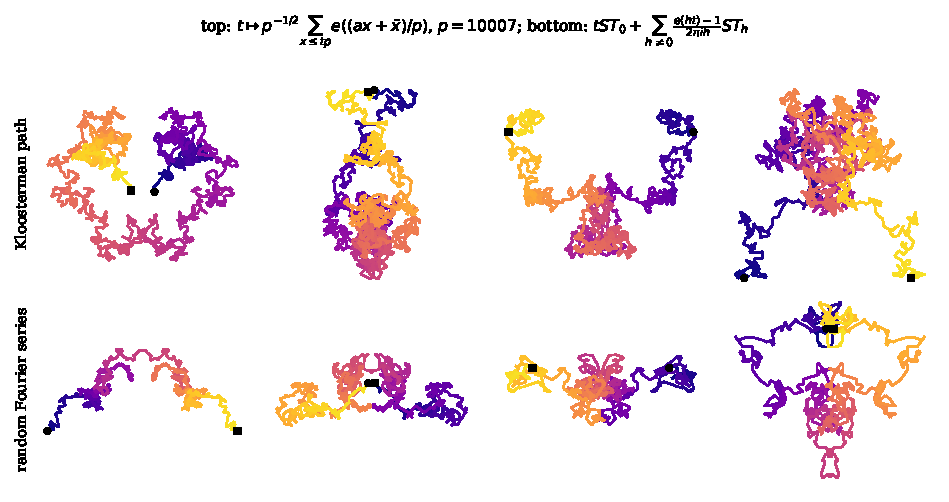
\includegraphics[width=\textwidth]{figs/kloosterman_paths.pdf}
\caption{Top: Kloosterman paths $t\mapsto p^{-1/2}\sum_{x\le t(p-1)}e((ax+\bar x)/p)$ in the complex plane for four values of $a$, $p=10007$, coloured by $t$. Bottom: four samples of the random Fourier series $K(t)$ of Definition~\ref{def:06bK}. Every path starts at $0$ and ends on the real axis at a point of $[-2,2]$; its imaginary part is symmetric about $t=\frac12$, and the path is symmetric under reflection in the vertical line through the midpoint of its endpoints (Proposition~\ref{prop:06bcov}).}\label{fig:06bpaths}
\end{figure}

\subsection{Properties of the limit}

\begin{proposition}[Covariance and symmetry of $K$; this book]\label{prop:06bcov}\index{random Fourier series}
For $s,t\in[0,1]$,
\[
\E\,K(s)\overline{K(t)}=\min(s,t),\qquad\E\,K(s)K(t)=(s+t-1)_+ .
\]
Consequently $\mathrm{Var}\,\Re K(t)=\frac12\bigl(t+(2t-1)_+\bigr)$, $\mathrm{Var}\,\Im K(t)=\frac12\bigl(t-(2t-1)_+\bigr)$, and $\Re K(t)$, $\Im K(t)$ are uncorrelated. Moreover, almost surely,
\[
K(1-t)=K(1)-\overline{K(t)}\qquad(0\le t\le1),
\]
so $\Im K(1-t)=\Im K(t)$, $K(1)=2\Re K(\frac12)=\mathrm{ST}_0$, and $\Im K(0)=\Im K(1)=0$.
\end{proposition}

\begin{proof}
Since the $\mathrm{ST}_h$ are independent, real, centred and of variance one, $\E K(s)\overline{K(t)}=\sum_hc_h(s)\overline{c_h(t)}$ and $\E K(s)K(t)=\sum_hc_h(s)c_h(t)$. With $f=\mathbb{I}_{[0,s]}$ and $g=\mathbb{I}_{[0,t]}$ we have $c_h(s)=\overline{\hat f(h)}$, so Parseval gives $\sum_h\overline{\hat f(h)}\hat g(h)=\int_0^1fg=\min(s,t)$. For the second identity, $\hat g(h)=\overline{\hat{\tilde g}(h)}$ with $\tilde g(u)=g(-u)$ on $\R/\Z$, so $\sum_h\overline{\hat f(h)}\,\overline{\hat g(h)}=\sum_h\overline{\hat f(h)}\hat{\tilde g}(h)=\int_0^1f(u)g(-u)\,du$, the length of $[0,s]\cap[1-t,1]$, which is $(s+t-1)_+$. Both sums are real, so the variances follow from $\mathrm{Var}\,\Re K=\frac12(\E|K|^2+\E K^2)$ and $\mathrm{Var}\,\Im K=\frac12(\E|K|^2-\E K^2)$, and the covariance of the real and imaginary parts is $\frac12\Im\E K^2=0$. For the symmetry, $e(h(1-t))=e(-ht)$ gives $c_h(1-t)=-\overline{c_h(t)}$ for $h\ne0$ and $c_h(1)=0$; summing term by term, $K(1-t)=(1-t)\mathrm{ST}_0-\overline{(K(t)-t\,\mathrm{ST}_0)}=\mathrm{ST}_0-\overline{K(t)}$, and $K(1)=\mathrm{ST}_0$.
\end{proof}

At $t=\frac14$ the formulas of Proposition~\ref{prop:06bcov} give $\frac18$ and $\frac18$, against the observed path variances $0.1234$ and $0.1249$, and at $t=\frac34$ they give $\frac58$ and $\frac18$, against $0.6308$ and $0.1249$; the two observed imaginary variances coincide, as the symmetry below forces already at finite $p$. The limits of the exact second moments in Proposition~\ref{prop:06bsecond}, $\E|S_p|^2\to t$ and $\E S_p^2\to(2t-1)_+$, are exactly these covariances at $s=t$, and the same computation with two intervals gives $\min(s,t)$ and $(s+t-1)_+$ for $s\ne t$: the second order structure of the paths agrees with that of $K$ unconditionally, without Katz's theorem.

The arithmetic meaning of the symmetry is simple: $x\mapsto p-x$ maps $e((ax+\bar x)/p)$ to its conjugate, so $K_p(a,1-t)=K_p(a,1)-\overline{K_p(a,t)}$ for all $t$. The second half of a Kloosterman path is therefore the mirror image of the first half in the vertical line $\Re z=\mathrm{Kl}(a;p)/(2\sqrt p)$, which is the symmetry visible in every path of Figure~\ref{fig:06bpaths}.

\begin{proposition}[Unboundedness and a Gaussian tail bound; this book]\label{prop:06btail}
The random variable $\Im K(\frac12)=\frac1\pi\sum_{h\ \mathrm{odd}}\mathrm{ST}_h/h$ is unbounded above and below, and for every $M>0$,
\[
\Prob\bigl(\Im K(\tfrac12)>M\bigr)\le e^{-2M^2},
\]
the Chernoff bound of a centred Gaussian variable with the same variance $\frac14$. More generally, every real random variable $X=\sum_h\gamma_h\mathrm{ST}_h$ with $\sum_h\gamma_h^2<\infty$, in particular every real linear combination of the real and imaginary parts of finitely many values of $K$, satisfies $\E e^{\lambda X}\le e^{\lambda^2\mathrm{Var}(X)/2}$ for all real $\lambda$.
\end{proposition}

\begin{proof}
At $t=\frac12$, $c_h=((-1)^h-1)/(2\pi ih)$ vanishes for even $h\ne0$ and equals $i/(\pi h)$ for odd $h$, which gives the formula; pairing $h$ with $-h$, $\Im K(\frac12)=\frac1\pi\sum_{h>0\ \mathrm{odd}}(\mathrm{ST}_h-\mathrm{ST}_{-h})/h$. Given $M$, choose $N$ with $\frac{3}{\pi}\sum_{h\le N,\ h\ \mathrm{odd}}\frac1h>M+1$, possible since the harmonic series over odd integers diverges. With positive probability $\mathrm{ST}_h>1.5$ and $\mathrm{ST}_{-h}<-1.5$ for all odd $h\le N$, so the partial sum exceeds $M+1$. The remainder is independent of this event and symmetric, so it is nonnegative with probability at least $\frac12$. Hence $\Prob(\Im K(\frac12)>M+1)>0$, and the law is symmetric. For the tail, the law $\ST$ is subgaussian with variance proxy equal to its variance: its odd moments vanish and its even moments are the Catalan numbers $C_k=(2k)!/(k!\,(k+1)!)$, so
\[
\E e^{\lambda\mathrm{ST}_h}=\sum_{k\ge0}\frac{\lambda^{2k}}{k!\,(k+1)!}\le\sum_{k\ge0}\frac{\lambda^{2k}}{2^kk!}=e^{\lambda^2/2},
\]
because $2^k\le(k+1)!$. For $X=\sum_h\gamma_h\mathrm{ST}_h$, independence gives $\E e^{\lambda X_N}\le e^{\lambda^2\sum_{|h|\le N}\gamma_h^2/2}$ for the partial sums $X_N$, which converge to $X$ almost surely, and Fatou's lemma gives $\E e^{\lambda X}\le e^{\lambda^2\mathrm{Var}(X)/2}$, since $\mathrm{Var}(X)=\sum_h\gamma_h^2$. For $\Im K(\frac12)$ we have $\gamma_h=1/(\pi h)$ for odd $h$ and $\sum_{h\ \mathrm{odd}}\gamma_h^2=\frac{2}{\pi^2}\cdot\frac{\pi^2}{8}=\frac14$, and Chernoff's bound with $\lambda=4M$ gives $\Prob(\Im K(\frac12)>M)\le e^{-4M^2+2M^2}=e^{-2M^2}$.
\end{proof}

So although each normalised Kloosterman sum lies in $[-2,2]$, the limit of the partial sums is unbounded, consistent with the fact that partial sums of such exponential sums can be as large as a constant times $\sqrt p\log\log p$; for Birch sums Lamzouri showed that some partial sum reaches $(\frac2\pi+o(1))\sqrt p\log\log p$ \cite{lamzouri2020}. The true tails are much thinner than Gaussian. Kowalski and Sawin prove that for $0<t<1$ there is $c=c(t)>0$ with
\[
c^{-1}\exp\bigl(-\exp(cM)\bigr)\le\Prob\bigl(|\Im K(t)|\ge M\bigr)\le c\exp\bigl(-\exp(M/c)\bigr)\quad(M>0),
\]
the same bounds for $|\Re K(t)|$ when $t\ne\frac12$, and bounds of the same shape for $\|K\|_\infty$ \cite{kowalskisawin2016}. For the maximum of the partial sums at finite $p$, Lamzouri obtained nearly matching bounds of this type for Birch sums \cite{lamzouri2020}, and Autissier, Bonolis and Lamzouri showed, for Birch sums and for the two parameter Kloosterman family, that the proportion of parameters for which the maximum exceeds $V\sqrt p$ is $\exp(-\exp(\pi V/2+O(1)))$, uniformly for $V$ up to about $\frac2\pi\log\log p$; for the further families of trace functions that they treat, whose normalised Fourier transforms take values in $[-N,N]$, they prove the same with $\frac\pi2$ replaced by $\frac\pi N$ and the range by $\frac N\pi\log\log p$ \cite{abl2021}.

\section{Probabilistic interpretation}\label{sec:06bprob}

\paragraph{A Sato Tate Brownian motion.} Proposition~\ref{prop:06bcov} says that on $[0,\frac12]$ the process $K$ has exactly the second order structure of a standard complex Brownian motion $Z$: $\E K(s)\overline{K(t)}=\min(s,t)$ and $\E K(s)K(t)=0$ for $s,t\le\frac12$. On $[\frac12,1]$ it is determined by its first half through the reflection $K(t)=2\Re K(\frac12)-\overline{K(1-t)}$. The Gaussian process with the same covariance is therefore complex Brownian motion on $[0,\frac12]$ folded back on itself: the imaginary part is a Brownian path on $[0,\frac12]$ followed by its time reversal, so it is pinned at $0$ at both ends like a bridge, and the real part is a Brownian path followed by its reflection through the midpoint value, ending at $2\Re Z(\frac12)$, a centred Gaussian of variance one. The Kloosterman process differs from this Gaussian model in two visible ways. Its endpoint $K(1)=\mathrm{ST}_0$ is semicircular, hence bounded, and its marginals are not Gaussian although their tails are subgaussian (Proposition~\ref{prop:06btail}), indeed doubly exponential. The three processes are one series with three choices of coefficients. With independent standard complex Gaussian coefficients ($\E|\zeta_h|^2=1$, $\E\zeta_h^2=0$) the series $\sum_hc_h(t)\zeta_h$ is a centred complex Gaussian process with covariances $\min(s,t)$ and $0$, by the proof of Proposition~\ref{prop:06bcov}, that is, a standard complex Brownian motion on $[0,1]$; with independent real standard Gaussian coefficients it is the folded process just described (Exercise~\ref{ex:06bgauss}); and with independent real Sato Tate coefficients, the traces of independent Haar elements of $\SU(2)$, it is $K$. In this sense $K$ is a Sato Tate Brownian motion.

\paragraph{Relation to random matrices.} Writing $\mathrm{ST}_h=\tr g_h$ with $g_h$ independent Haar elements of $\SU(2)$, the limit is a linear statistic of an infinite sequence of independent random matrices. Other one variable sums lead to other groups. For the additive twists $x\mapsto\mathrm{Kl}^{(r)}(\overline{ax};p)\,e(bx/p)$ of the hyper Kloosterman sums $\mathrm{Kl}^{(r)}(c;p)=\sum_{y_1\cdots y_r=c}e((y_1+\dots+y_r)/p)$, the discrete Fourier transforms are, after normalisation, the hyper Kloosterman sums $\mathrm{Kl}^{(r+1)}(\bar a(b+h);p)$ for $h\ne-b$, so Katz's monodromy computation makes the coefficients of the limit traces of Haar elements of $\USp(r+1)$ when $r$ is odd; for odd $r\ge3$ these are among the families of Autissier, Bonolis and Lamzouri recalled in Section~\ref{sec:06bpaths}, with $N=r+1$. For prime power moduli Ricotta and Royer found a limit of the same shape whose coefficients have an atom of mass $\frac12$ at $0$ and an arcsine part \cite{ricottaroyer2018}. This law is the measure $\mu_{\mathrm{CM}}$ of elliptic curves with complex multiplication (Chapter~\ref{ch:04}), because Kloosterman sums to prime power moduli have an elementary evaluation: for odd $p$, modulus $p^k$ with $k\ge2$ and parameters prime to $p$, they vanish unless the product of the parameters is a square modulo $p$, and are otherwise, up to sign, $p^{k/2}$ times twice the cosine of an explicit angle.

\paragraph{Open questions.} We record four.
\begin{enumerate}
\item The law of $\|K\|_\infty$ is not known in closed form. Autissier, Bonolis and Lamzouri determine its tail up to the constant in the exponent, $\Prob(\|K\|_\infty>V)=\exp(-\exp(\pi V/2+O(1)))$ for large $V$ \cite{abl2021}, but the distribution function, and even its mean ($1.138$ in our simulation), have no formula.
\item Extreme values. In the two parameter family the normalised maximum of the partial sums is $O(\log p)$ for every $(a,b)$ by the completion method, and exceeds $(\frac2\pi+o(1))\log\log p$ for many $(a,b)$ \cite{abl2021}. Whether it is $O(\log\log p)$ for all $(a,b)$, which is what the estimate of Autissier, Bonolis and Lamzouri would give if it held for all $V$, is open; they show that the corresponding bound fails for some families of periodic functions to which their theorem applies, although these families, unlike Kloosterman sums, are not uniformly bounded.
\item For the one parameter family, convergence in law in $C([0,1])$ depends on estimates for short Kloosterman sums averaged over the parameter that are not known (see the discussion of tightness above).
\item Horizontal paths. Fix an integer $a\ne0$ and let $p$ be uniform among the primes up to $x$. Do the paths $K_p(a,\cdot)$ converge in finite dimensional distributions, as $x\to\infty$, to $K-c_a\mathrm{ST}_a$? For fixed $a$ the term $h=a$ of \eqref{eq:06bcompletion} is $-\alpha_p(a,t)/\sqrt p$, so one Sato Tate coefficient disappears, as in the second parametrisation. The endpoint $K_p(a,1)=2\cos\theta_{p,a}$ alone is the subject of Conjecture~\ref{conj:06bhorizontal}, and the finite dimensional distributions would also need the angles $\theta_{p,a-h}$ at distinct shifts $h\ne a$ to become independent as $p$ varies.
\end{enumerate}

\section{Notes}

Kloosterman introduced his sums in 1926 to treat quaternary quadratic forms by the circle method, obtaining a bound of order $p^{3/4}$ \cite{kloosterman1926}. Weil's paper \cite{weil1948b} deduced $2\sqrt p$ from his proof of the Riemann hypothesis for curves over finite fields \cite{weil1948}; Stepanov's method \cite{stepanov1969}, in Bombieri's formulation \cite{bombieri1974}, gives an elementary proof. The theory of Kloosterman sheaves, their monodromy, and the equidistribution theorem are in Katz's monograph \cite{katz1988}; Deligne's equidistribution theorem is in Weil II \cite{deligne1980}, and the Goursat Kolchin Ribet criterion is in \cite{katz1990}. Katz and Sarnak \cite{katzsarnak1999} develop the general passage from monodromy to random matrices used in Chapter~\ref{ch:06}. Iwaniec and Kowalski \cite{iwanieckowalski2004} treat exponential sums over finite fields, Kloosterman sums included, in Chapter 11 and sums of Kloosterman sums with the Kuznetsov formula in Chapter 16; Iwaniec's book \cite{iwaniec2002} is the standard reference for the spectral theory. The Kuznetsov formula is due independently to Bruggeman \cite{bruggeman1978} and Kuznetsov \cite{kuznetsov1980}; Deshouillers and Iwaniec \cite{deshouillersiwaniec1982} combined it with large sieve inequalities for Fourier coefficients and turned it into a standard tool of analytic number theory. Selberg's 3/16 theorem and the Kloosterman zeta function are in \cite{selberg1965}, and the record $\frac{975}{4096}$ is in the appendix of Kim and Sarnak to \cite{kimsarnak2003}. The paths, the completion formula of Lemma~\ref{lem:06bcompletion} and the observation that the parametrisation $e((x+a\bar x)/p)$ loses one coefficient of the limit are due to Kowalski and Sawin \cite{kowalskisawin2016}, who describe the support of the limit in \cite{kowalskisawin2017}. Lemma~\ref{lem:06btail}, Proposition~\ref{prop:06bsecond}, Corollary~\ref{cor:06bdeficit}, Proposition~\ref{prop:06bcov} and Proposition~\ref{prop:06btail} are our own formulations, with complete proofs, of facts that are implicit in or easily derived from their work; the tail bound of Proposition~\ref{prop:06btail} is far weaker than their doubly exponential estimates. Lamzouri \cite{lamzouri2020} and Autissier, Bonolis and Lamzouri \cite{abl2021} study the maximum of the partial sums at finite $p$, and Ricotta and Royer \cite{ricottaroyer2018} the paths for prime power moduli.

\section{Exercises}

\begin{enumerate}
\item\label{ex:06bbasic} Show that $\mathrm{Kl}(a,b;p)$ is real, that $\mathrm{Kl}(a,b;p)=\mathrm{Kl}(1,ab;p)$ for $a\ne0$, and that $\mathrm{Kl}(a,b;p)=\mathrm{Kl}(b,a;p)$. Deduce that for $ab\ne0$ the sum depends only on $ab$.
\item Show that $\sum_{x\in\mathbb{F}_p^\times}e(c\bar x/p)=-1$ for $c\ne0$ (a Ramanujan sum), and deduce $\mathrm{Kl}(0;p)=-1$ and $\sum_{a\in\mathbb{F}_p^\times}\mathrm{Kl}(a;p)=1$. Let $m_2$ and $m_4$ be the empirical second and fourth moments of $x_{p,a}$ over $a\in\mathbb{F}_p^\times$ (Proposition~\ref{prop:06bmoments}). Using the Paley Zygmund inequality $\Prob(Z>\theta\,\E Z)\ge(1-\theta)^2(\E Z)^2/\E Z^2$ for $Z\ge0$ and $0\le\theta\le1$, show that the proportion of $a$ with $|\mathrm{Kl}(a;p)|>\frac12\sqrt p$ is at least $(m_2-\frac14)^2/m_4$, which tends to $\frac9{32}$. Compare with the Sato Tate value $\ST(\{x:|x|>\frac12\})=0.685$.
\item For $p=5$, compute by hand $\mathrm{Kl}(1;5)=\frac{3-\sqrt5}2$, $\mathrm{Kl}(2;5)=-1-\sqrt5$, $\mathrm{Kl}(3;5)=\sqrt5-1$, $\mathrm{Kl}(4;5)=\frac{3+\sqrt5}2$. Check Weil's bound $2\sqrt5$ and the three identities of Proposition~\ref{prop:06bmoments} (the fourth moment is $159$), and find the Kloosterman angles.
\item\label{ex:06bweilL} Suppose $L_a(T)=1+\mathrm{Kl}(a;p)T+pT^2=(1-\alpha T)(1-\beta T)$ and $\mathrm{Kl}_n(a)=-(\alpha^n+\beta^n)$. Show that $\mathrm{Kl}_2(a)=2p-\mathrm{Kl}(a;p)^2$. Show that if $|\mathrm{Kl}_n(a)|\le Cp^{n/2}$ for all $n$, with $C$ independent of $n$, then $|\alpha|=|\beta|=\sqrt p$. (Hint: consider the radius of convergence of $\sum_n\mathrm{Kl}_n(a)T^n$.)
\item (Probabilistic.) Compute $\mathrm{Var}\,\Re K(t)$ and $\mathrm{Var}\,\Im K(t)$ directly from the series, using $\sum_{h\ne0}\frac{\sin^2(\pi ht)}{\pi^2h^2}=t(1-t)$ for $0\le t\le1$, which follows from the Fourier expansion of the Bernoulli polynomial $B_2(t)=t^2-t+\frac16$. Check the answer against Proposition~\ref{prop:06bcov}, and show that $\mathrm{Var}\,\Im K(t)=\frac12\min(t,1-t)$, maximal at $t=\frac12$.
\item\label{ex:06bgauss} (Probabilistic.) Let $\xi_h$ be independent real standard Gaussians and $B(t)=\sum_hc_h(t)\xi_h$. Show that $B$ is a complex Gaussian process with the covariance of Proposition~\ref{prop:06bcov}, identify it in terms of a standard complex Brownian motion on $[0,\frac12]$ as in Section~\ref{sec:06bprob}, and compute $\Prob(\Im B(\frac12)>M)$. Compare with the bound $e^{-2M^2}$ of Proposition~\ref{prop:06btail}. Show that if the $\xi_h$ are replaced by independent standard complex Gaussians, the same series is a standard complex Brownian motion on $[0,1]$.
\end{enumerate}

\section{Open computational problems}

\begin{compproblem}[Horizontal statistics of Kloosterman angles]
Objective: test Conjecture~\ref{conj:06bhorizontal} for $a=1$ and a few other small $a$. Objects: $\mathrm{Kl}(a;p)/\sqrt p$ for all primes $p\le10^8$ and for a random sample of $10^5$ primes in $[10^8,10^9]$. Route: each sum costs $O(p)$ operations with modular inversion by a batched Montgomery trick; GPU kernels accumulating $\cos(2\pi(x+a\bar x)/p)$ in double precision, with compensated summation; cross check against PARI/GP at small $p$. Deliverable: Weyl averages $\pi(x)^{-1}\sum_{p\le x}U_n(x_p/2)$ for $n\le20$ as functions of $x$, $\sqrt{\pi(x)}$ times the Kolmogorov distance to $\ST$, and the counts of positive and negative values. Why it matters: unlike Satake angles of a fixed modular form, Kloosterman angles at varying primes come from no known global object, so no automorphic proof of the horizontal law is in sight, and the data measure whether they are nevertheless as random as Satake angles.
\end{compproblem}

\begin{compproblem}[Law of the maximum of Kloosterman paths]
Objective: estimate the distribution of $\|K_p(a,\cdot)\|_\infty$ and compare it with that of $\|K\|_\infty$. Objects: all $a\in\mathbb{F}_p^\times$ for a sequence of primes $p$ up to $10^6$ (about $10^{12}$ terms for the largest), in both parametrisations of Proposition~\ref{prop:06bsecond} (the second should be compared with $K-c_1\mathrm{ST}_1$), and $10^7$ samples of the random Fourier series truncated at $|h|\le10^4$. Route: cumulative sums of $e((ax+\bar x)/p)$ from a table of inverses, vectorised over $a$ on GPUs, keeping only the running maximum of the modulus; the series evaluated on a fine grid by fast Fourier transforms. Deliverable: empirical distribution functions and upper tails of the maxima, a fit of $\log(-\log\Prob(\|K\|_\infty>V))$ against $V$ to measure the doubly exponential rate, and two sample tests by $p$. Why it matters: agreement at large $p$ is evidence for convergence in $C([0,1])$ for the one parameter family, which is not proved, and the fitted slope can be compared with the value $\frac\pi2$ of Autissier, Bonolis and Lamzouri \cite{abl2021}.
\end{compproblem}

\begin{compproblem}[Sums of Kloosterman sums and the spectral gap]
Objective: measure $\Sigma_N(x)=\sum_{c\le x,\ N\mid c}S(m,n;c)/c$ against Conjecture~\ref{conj:06blinnik}. Objects: $m,n\le10$, levels $N\le100$, and $x$ up to $10^7$. Route: compute $S(m,n;p)$ for primes $p\le x$ on GPUs, obtain prime power moduli from the explicit evaluations, and assemble composite moduli by twisted multiplicativity; smooth the sums with a fixed weight. Deliverable: plots of $\Sigma_N(x)$ against $\log x$, fitted growth exponents with confidence bands, and a comparison of $|\Sigma_N(x)|^2$ with $V_N(x)=\sum_{c\le x,\ N\mid c}S(m,n;c)^2/c^2$, the variance of the model in which the terms carry independent random signs. Why it matters: Conjecture~\ref{conj:06blinnik} is open even for $N=1$, where Kuznetsov's exponent $\frac16$ stands, and an exceptional eigenvalue $s(1-s)$ of $\Gamma_0(N)$ would produce a drift of order $x^{2s-1}$; the experiment turns Selberg's eigenvalue conjecture into a test for the absence of drift in an arithmetic random walk.
\end{compproblem}

\begin{compproblem}[Birch paths]
Objective: study the paths $t\mapsto p^{-1/2}\sum_{0\le x\le tp}e((ax+bx^3)/p)$ for the one parameter family ($b=1$) and the two parameter family $(a,b)$. Objects: all $a$ (and $10^6$ random pairs $(a,b)$) for a sequence of primes up to $10^6$. Route: as in the previous problems, with the cubic phase computed exactly modulo $p$. Deliverable: Kolmogorov Smirnov comparisons with the random Fourier series of Kowalski and Sawin at fixed $t$, the variance functions $\mathrm{Var}\,\Re$ and $\mathrm{Var}\,\Im$ against the formulas of Proposition~\ref{prop:06bcov} (for $b=1$ the limit is again $K$ \cite{kowalskisawin2016}), the law of the maximum, and a check of the vertical Sato Tate law for the complete sums. Why it matters: Birch sums are the case in which convergence in $C([0,1])$ is a theorem, so they calibrate the numerical methods used for Kloosterman paths.
\end{compproblem}
